
\chapter{Regular Expressions \label{chapter:regular-expressions}}

\begin{figure}[h]  % 'h' suggests placement "here"
\centering
  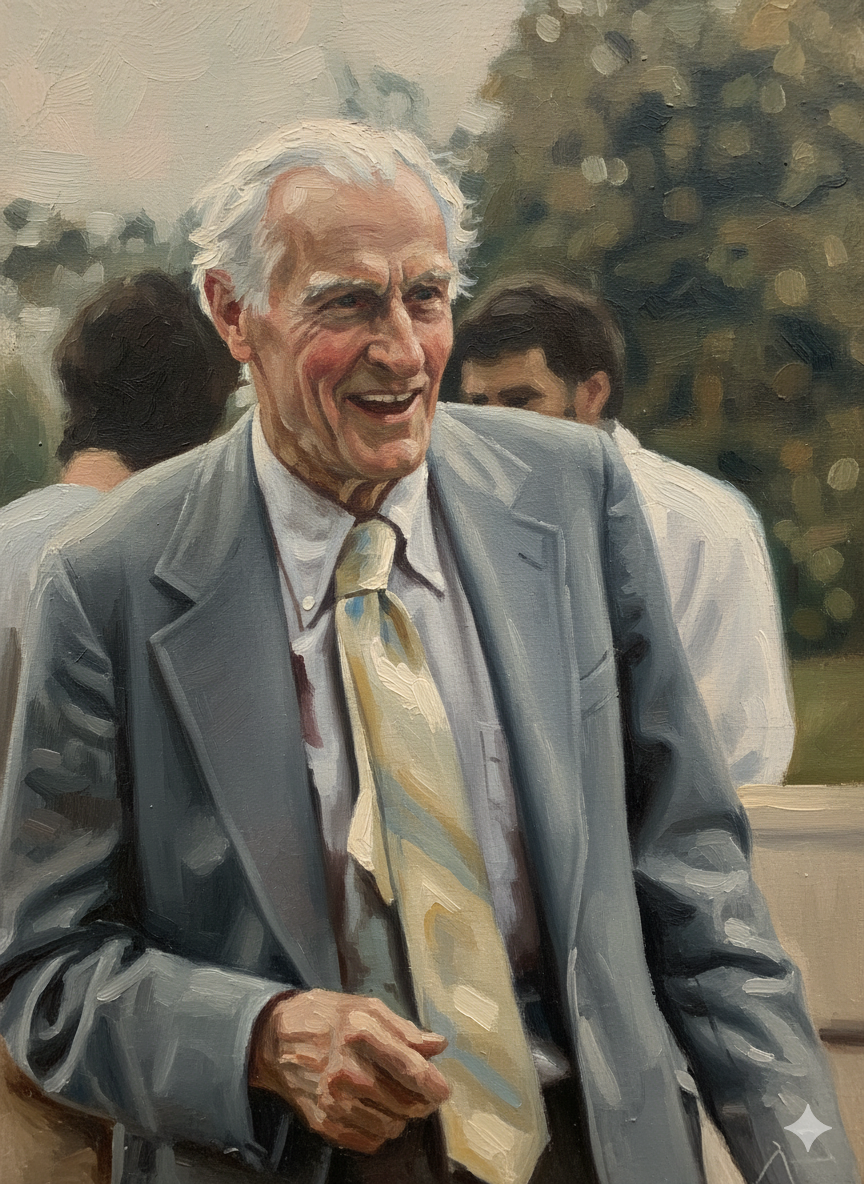
\includegraphics[width=10.5cm]{Abbildungen/Stephen_Cole_Kleene.png}
\caption{Stephen Cole Kleene, the father of regular languages.}
\label{fig:chapter-image}
\end{figure}

\href{http://en.wikipedia.org/wiki/Regular_expression}{\emph{Regular expressions}} \index{regular expression}
are linguistic constructs designed to specify formal languages simple enough to be recognized by a
\blue{finite state machine}.  These machines will be introduced in Chapter \ref{chapter:finite-state-machines}.
At the core, regular expressions enable the specification of:  
\begin{enumerate}[(a)]
\item Alternatives among different options,
\item Concatenation of elements, and
\item Repetition of elements.
\end{enumerate}

Regular expressions form the backbone of many modern scripting languages. For instance, the initial surge in
the popularity of the programming language \href{http://en.wikipedia.org/wiki/Perl}{\textsl{Perl}} can be
largely attributed to its efficient handling of regular expressions. Today,  most popular high-level
programming languages (e.g.~\textsl{Python}, \texttt{C++}, \textsl{Java}, \texttt{C\#}, \texttt{JavaScript},
\texttt{PHP}, \texttt{Ruby}) support regular expressions.  In the programming language \texttt{C} regular
expressions are available via the \textsc{Posix} library.  

Moreover, various \textsc{Unix} utilities, including \href{http://en.wikipedia.org/wiki/Grep}{\texttt{grep}},
\href{http://en.wikipedia.org/wiki/Sed}{\texttt{sed}}, and
\href{http://en.wikipedia.org/wiki/Awk}{\texttt{awk}}, are based on regular
expressions. Consequently, proficiency in regular expressions is indispensable for a budding computer scientist.

In this chapter, we will introduce a definition of regular expressions that is more concise than those typically found in programming languages. This streamlined definition will facilitate our theoretical examination of regular languages in Chapters \ref{chapter:finite-state-machines} and \ref{chapter:regular-languages}. The syntax of regular expressions as used in \textsl{Python} will be covered in the subsequent chapter.

\section{Preliminary Definitions}
Before delving into the syntax and semantics of regular expressions, we need to introduce some preliminary definitions.

\begin{Definition}[Product of Languages]
  Given an alphabet $ \Sigma $ and formal languages $ L_1, L_2 \subseteq \Sigma^* $, the
  \blue{product}\index{product of languages} of $ L_1 $ and $ L_2 $ is denoted as $ L_1 \cdot L_2 $ and
  is defined as the set of all concatenations $ w_1 \cdot w_2 $ where $ w_1 \in L_1 $ and $ w_2 \in L_2
  $. Formally,  
\\[0.2cm]
\hspace*{1.3cm}
$ L_1 \cdot L_2 := \{ w_1 \cdot w_2 \mid w_1 \in L_1 \land w_2 \in L_2 \}$. \eox 
\end{Definition}

\exampleEng
Suppose $ \Sigma = \{ \texttt{a}, \texttt{b}, \texttt{c} \} $ and $ L_1 $ and $ L_2 $ are given by
\[
L_1 = \{ \texttt{ab}, \texttt{bc} \} \quad \text{and} \quad L_2 = \{ \texttt{ac}, \texttt{cb} \},
\]
then $ L_1 \cdot L_2 = \{ \texttt{abac}, \texttt{abcb}, \texttt{bcac}, \texttt{bccb} \} $. \eox


\begin{Definition}[Power of a Language]\index{power of a language}
Let $ \Sigma $ be an alphabet, $ L \subseteq \Sigma^* $ a formal language, and $ n \in \mathbb{N} $. The $ n $-th \blue{power} of $ L $, denoted as $ L^n $, is defined inductively as follows:
\begin{enumerate}
\item[B.C.:] $ n = 0 $:

             $ L^0 := \{ \lambda \} $, \quad where $ \lambda $ is the empty string.
\item[I.S.:] $ n \mapsto n + 1 $:
             
             $ L^{n+1} = L^n \cdot L $. \eox
\end{enumerate}
\end{Definition}

\exampleEng
For $ \Sigma = \{ \texttt{a}, \texttt{b} \} $ and $ L = \{ \texttt{ab}, \texttt{ba} \} $, we find:
\begin{enumerate}[(a)]
\item $ L^0 = \{ \lambda \} $,
\item $ L^1 = L $,
\item $ L^2 = \{ \texttt{abab}, \texttt{abba}, \texttt{baab}, \texttt{baba} \} $. \eox
\end{enumerate}

\begin{Definition}[Kleene Closure]
  Given an alphabet $ \Sigma $ and a formal language $ L \subseteq \Sigma^* $, the \blue{Kleene
    closure}\index{Kleene closure} of $ L $, denoted as $ L^* $, is the union of all $ L^n $ for $ n \in \mathbb{N} $:
  \[
  L^* := \bigcup_{n \in \mathbb{N}} L^n = L^0 \cup L^1 \cup L^2 \cup \cdots
  \]
  Note that $ \lambda \in L^* $, so $ L^* $ is never empty, even when $ L = \{\} $.

  The Kleene closure is named after \href{https://en.wikipedia.org/wiki/Stephen_Cole_Kleene}{Stephen Cole Kleene}
  (1909--1994), who invented regular expressions.
  \eox
\end{Definition}

The previous example highlights that the Kleene closure of a finite language can be infinite. Specifically, 
$L^*$ will be infinite whenever $L$ contains a string different from $\lambda$. 

\begin{Definition}[Power of a string, $s^n$]\index{power of a string}
For a string $ s $ and a non-negative integer $ n \in \mathbb{N} $, the expression $ s^n $ is defined inductively:
\begin{enumerate}
\item[B.C.:] $ n = 0 $:

             $ s^0 := \lambda $.
\item[I.S.:] $ n \mapsto n + 1 $:

             $ s^{n+1} := s^n \cdot s $,  \quad where $ s^n \cdot s $ represents the concatenation of $ s^n $ and $ s $.
\eox
\end{enumerate}
\end{Definition}

\exampleEng
Let $ \Sigma = \{ \texttt{a}, \texttt{b} \} $ and $ L = \{ \texttt{a} \} $. Then
\[
L^* = \{ \texttt{a}^n \mid n \in \mathbb{N} \},
\]
where $ \texttt{a}^n $ represents a string of $ n $ consecutive \texttt{a}'s. \eox



\section{The Formal Definition of Regular Expressions}
We proceed to define the set of regular expressions for a given alphabet $ \Sigma $. This set is denoted as
$ \texttt{RegExp}_\Sigma $, and is defined inductively. Simultaneously, we define the function 
\\[0.2cm]
\hspace*{1.3cm}
$L: \texttt{RegExp}_\Sigma \rightarrow 2^{\Sigma^*}$,
\\[0.2cm]
which interprets each regular expression $ r $ as a formal language $ L(r) \in 2^{\Sigma^*} $.\footnote{
  Given a set $ M $, the \blue{power set} of $ M $, i.e., the set of all subsets of $ M $, is denoted as $ 2^M $.
}
\pagebreak

\begin{Definition}[Regular Expressions, Stephen Cole Kleene] \index{regular expression}
  The set $ \texttt{RegExp}_\Sigma $ of \blue{regular expressions} on the alphabet $ \Sigma $ is defined inductively as follows:
  \begin{enumerate}
  \item $\emptyset \in \texttt{RegExp}_\Sigma$ \index{$\emptyset$}

        The regular expression $\emptyset$ denotes the empty language, we have
        \\[0.2cm]
        \hspace*{1.3cm}
        $L(\emptyset) := \{\}$.

        In order to avoid confusion we assume that the symbol $\emptyset$ is \underline{not} a member of the
        alphabet $\Sigma$, i.e.~we have $\emptyset \not\in \Sigma$.
  \item $\varepsilon \in \texttt{RegExp}_\Sigma$ \index{$\varepsilon$}

        The regular expression $\varepsilon$ denotes the language that only contains the empty
        string $\lambda$: 
        \\[0.2cm]
        \hspace*{1.3cm}
        $L(\varepsilon) := \{ \lambda \}$.

        Furthermore, we assume that $\varepsilon \not\in \Sigma$.
  \item $c \in \Sigma \rightarrow c \in \texttt{RegExp}_\Sigma$.

        Every character from the alphabet $\Sigma$ is a regular expression.  This expression denotes
        the language that contains only the string $c$:
        \\[0.2cm]
        \hspace*{1.3cm}
        $L(c) := \{ c \}$.
        \\[0.2cm]
        Observe that we identify characters with strings of length one.
  \item $r_1 \in \texttt{RegExp}_\Sigma \wedge r_2 \in \texttt{RegExp}_\Sigma
         \rightarrow r_1 + r_2 \in \texttt{RegExp}_\Sigma$

        Starting from two regular expressions $r_1$ and $r_2$ we can use the  infix operator
        ``$+$'' to build a new regular expression.  This regular expression denotes the union of 
        the languages described by $r_1$ and $r_2$:
        \\[0.2cm]
        \hspace*{1.3cm}
        $L(r_1 + r_2) := L(r_1) \cup L(r_2)$.

        We have to assume that the symbol  ``\texttt{+}'' does not occur in the alphabet $\Sigma$, i.e.~we have  $\squoted{+} \not\in \Sigma$.
  \item $r_1 \in \texttt{RegExp}_\Sigma \wedge r_2 \in \texttt{RegExp}_\Sigma 
         \rightarrow r_1 \cdot r_2 \in \texttt{RegExp}_\Sigma$

        Starting from the regular expression $r_1$ and $r_2$ we can use the  infix operator
        ``$\cdot$'' to build a new regular expression.  This regular expression denotes
        the product of the languages of $r_1$ and $r_2$:
        \\[0.2cm]
        \hspace*{1.3cm}
        $L(r_1 \cdot r_2) := L(r_1) \cdot L(r_2)$.

        We have to assume that the symbol ``$\cdot$'' does not occur in the alphabet $\Sigma$, i.e.~we have $\squoted{$\cdot$} \not\in \Sigma$.
  \item $r \in \texttt{RegExp}_\Sigma \rightarrow r^* \in \texttt{RegExp}_\Sigma$

        Given a regular expression $r$, the postfix operator
        ``$^*$'' can be used to create a new regular expression.  This new regular expression
        denotes the Kleene closure of the language described by  $r$:
        \\[0.2cm]
        \hspace*{1.3cm}
        $L(r^*) := \bigl(L(r)\bigr)^*$.

        We have to assume that $\squoted{$^*$} \not\in \Sigma$. 
  \item $r \in \texttt{RegExp}_\Sigma \rightarrow (r) \in \texttt{RegExp}_\Sigma$

        Regular expressions can be surrounded by parentheses.  This does not change the language
        denoted by the regular expression:
        \\[0.2cm]
        \hspace*{1.3cm}
        $L\bigl((r)\bigr) := L(r)$. 

        We have to assume that the parentheses  \qote{(} and \qote{)} do not occur
        in the alphabet $\Sigma$, i.e.~we have $\squoted{(} \not\in \Sigma$  and $\squoted{)} \not\in \Sigma$. \eox
  \end{enumerate}
\end{Definition}
Given the preceding definition, it is unclear whether we interpret the regular expression
\\[0.2cm]
\hspace*{1.3cm}
$\mathtt{a} + \mathtt{b} \cdot \mathtt{c}$
\\[0.2cm]
as either 
\\[0.2cm]
\hspace*{1.3cm}
$(\mathtt{a} + \mathtt{b}) \cdot \mathtt{c}$ \quad or instead as \quad $\mathtt{a} + (\mathtt{b} \cdot \mathtt{c})$.
\\[0.2cm]
To remove this ambiguity, we assign \blue{operator precedences} as follows:
\begin{enumerate}
\item The postfix operator ``$^*$'' has the highest precedence.
\item The infix operator ``$\cdot$'' has a lower precedence than the postfix operator ``$^*$'' but a higher precedence
      than the infix operator ``$+$''.
\item The infix operator ``$+$'' has the lowest precedence.
\end{enumerate}
With these conventions, the expression
\\[0.2cm]
\hspace*{1.3cm}
$\mathrm{a} + \mathrm{b} \cdot \mathrm{c}^*$
\\[0.2cm]
is interpreted as
\\[0.2cm]
\hspace*{1.3cm}
$\mathrm{a} + \bigl( \mathrm{b} \cdot (\mathrm{c}^*) \bigr)$.
\\[0.2cm]
\examplesEng
In the following examples, the alphabet $ \Sigma $ is defined as
\\[0.2cm]
\hspace*{1.3cm}
$\Sigma := \{ \texttt{a}, \texttt{b}, \texttt{c} \}$.
\begin{enumerate}
\item $ r_1 := (\texttt{a} + \texttt{b} + \texttt{c}) \cdot (\texttt{a} + \texttt{b} + \texttt{c}) $

      This expression $ r_1 $ denotes the set of all strings from $\Sigma^*$ that have length 2:
      \\[0.2cm]
      \hspace*{1.3cm}
      $ L(r_1) = \bigl\{ w \in \Sigma^* \bigm| |w| = 2 \bigr\}$.
\item $ r_2 := (\texttt{a} + \texttt{b} + \texttt{c}) \cdot (\texttt{a} + \texttt{b} + \texttt{c})^* $

      This expression $ r_2 $ denotes the set of all strings from $\Sigma^*$ that have at least length 1:
      \\[0.2cm]
      \hspace*{1.3cm}
      $L(r_2) = \bigl\{ w \in \Sigma^* \bigm|\, |w| \geq 1 \bigr\}$.
\item $ r_3 := (\texttt{b} + \texttt{c})^* \cdot \texttt{a} \cdot (\texttt{b} + \texttt{c})^* $

      This expression $ r_3 $ denotes the set of all strings from $\Sigma^*$ that have exactly one occurrence of the letter \texttt{a}:
      \\[0.2cm]
      \hspace*{1.3cm}
      $L(r_3) = \Bigl\{ w \in \Sigma^* \Bigm| \#\bigl\{i \in \mathbb{N} \bigm|\, w[i] = \texttt{a} \bigr\} = 1 \Bigr\}$. 
\item $ r_4 :=  (\texttt{b} + \texttt{c})^* \cdot \texttt{a} \cdot (\texttt{b} + \texttt{c})^* + (\texttt{a} + \texttt{c})^* \cdot \texttt{b} \cdot (\texttt{a} + \texttt{c})^* $

      This expression $ r_4 $ denotes the set of all strings from $\Sigma^*$ that either contain exactly one
      occurrence of the letter \texttt{a} or exactly one occurrence of the letter \texttt{b}: 
      \\[0.2cm]
      \hspace*{1.3cm}
      $L(r_4) = \Bigl\{ w \in \Sigma^* \bigm| \#\bigl\{i \in \mathbb{N} \bigm| w[i] = \texttt{a} \bigr\} = 1
      \Bigr\} \cup \Bigl\{ w \in \Sigma^* \bigm| \#\bigl\{i \in \mathbb{N} \bigm| w[i] = \texttt{b} \bigr\} = 1
      \Bigr\}$.  \eox
\end{enumerate}

\remarkEng
The syntax of regular expressions given here is the same as the syntax used in \cite{hopcroft:06}. However, the
syntax used for regular expressions in programming languages like \textsl{Python} differs. These differences
will be discussed later. 
\eox


\exerciseEng
\begin{enumerate}[(a)]
\item Assume $ \Sigma = \{ \mathtt{a}, \mathtt{b}, \mathtt{c} \} $. Define a regular expression for the language $ L \subseteq \Sigma^* $ that consists of those strings that contain at least one occurrence of the letter ``\texttt{a}'' and one occurrence of the letter ``\texttt{b}''.

\item Assume $ \Sigma = \{ 0, 1 \} $. Specify a regular expression for the language $ L \subseteq \Sigma^* $ that consists of those strings $ s $ such that the \href{https://dictionary.cambridge.org/dictionary/english/antepenultimate}{antepenultimate} character is the symbol ``$ 1 $''.

\item Again, assume $\Sigma = \{ 0, 1 \}$. Define a regular expression for the language $L \subseteq \Sigma^*$
      containing all those strings that do not contain the substring $ 110 $.  

% \solutionEng
% The regular expression $r$ that is sought for can be defined as 
% \\[0.2cm]
% \hspace*{1.3cm}
% $r = (0 + 1 \cdot 0)^* \cdot 1^*$.
% \\[0.2cm]
% First, it is quite obvious that the language $L(r)$ does not contain a string $w$ such that
% $w$ contains the substring $110$.  This is so because a character $1$ that is generated by the
% part $(0 + 1 \cdot 0)^*$ is immediately followed by a $0$.  Hence if $w$ contains the
% substring $110$, the first $1$ cannot originate from the regular expression $(0 + 1 \cdot 0)^*$.
% Furthermore, if the first $1$ of the substring 110 originates from the regular expression
% $1^*$, then there cannot be a $0$ following since the language generated by $1^*$ contains
% only ones.

% Second, assume that the string $w$ does not contain the substring $110$.  We have to show that
% $w \in L(r)$.  Now if the character $1$ does not occur in the
% string $w$, then $w$ is just a bunch of zeros and therefore $w$ can be generated by the
% regular expression $(0+1\cdot 0)^*$ and hence also by $(0 + 1  \cdot 0)^* \cdot 1^*$.  If the string $w$
% does contain the character $1$, there are two cases.
% \begin{enumerate}
% \item The first occurrence of $1$ is followed by a $0$.  Then the prefix of $w$ up to and
%       including this $0$ is generated by the regular expression $(0 + 1 \cdot 0)^*$.  The
%       remaining part of $w$ is shorter and, by induction, can be shown to be generated by 
%       $(0 + 1 \cdot 0)^* \cdot 1^*$.
% \item The first occurrence of $1$ is followed by another $1$.  In this case, the rest of $w$
%       must be made up of ones.  Hence, the part of $w$ starting with the first $1$ is
%       generated by $1^*$ and obviously the preceding zeros can all be generated by 
%       $(0 + 1 \cdot 0)^*$.
% \end{enumerate}
\item Again, assume $ \Sigma = \{0,1\} $. What is the language $ L $ generated by the regular expression 
      \\[0.2cm]
      \hspace*{1.3cm}
      $(1 + \varepsilon)\cdot(0\cdot 0^* \cdot 1)^* \cdot 0^*$? \eox

      % \solutionEng
      % This is the language $ L $ such that the strings in $ L $ do not contain the substring $ 11 $.
      % \eox
\end{enumerate}

\section{Algebraic Simplification of Regular Expressions}
Given two regular expressions $r_1$ and $r_2$, we use the notation
\\[0.2cm]
\hspace*{1.3cm}
$r_1 \doteq r_2 \quad \text{iff} \quad L(r_1) = L(r_2)$, \index{$\doteq$}
\\[0.2cm]
to indicate that $ r_1 $ and $ r_2 $ describe the same language. If the equation $ r_1 \doteq r_2 $
holds, then we refer to $ r_1 $ and $ r_2 $ as \blue{equivalent}.\index{equivalence of regular expressions} The
following algebraic laws hold: 
\begin{enumerate}[(a)]
\item $r_1 + r_2 \doteq r_2 + r_1$

      This equation is true because the union operator is commutative for sets:
      \\[0.2cm]
      \hspace*{1.3cm}
      $L(r_1 + r_2) = L(r_1) \cup L(r_2) = L(r_2) \cup L(r_1) = L(r_2 + r_1)$.
\item $(r_1 + r_2) + r_3 \doteq r_1 + (r_2 + r_3)$

      This equation is true because the union operator is associative for sets.
\item $(r_1 \cdot r_2) \cdot r_3 \doteq r_1 \cdot (r_2 \cdot r_3)$

      This equation is true because the concatenation of strings is associative, for any strings
      $u$, $v$, and $w$ we have
      \\[0.2cm]
      \hspace*{1.3cm}
      $(u v) w = u (v w)$.
      \\[0.2cm]
      This implies
      \\[0.2cm]
      \hspace*{1.3cm}
      $
      \begin{array}[t]{lcl}
        L\bigl( (r_1 \cdot r_2) \cdot r_3\bigr) 
        & = & \bigl\{ x w \bigm| x \in L(r_1 \cdot r_2) \wedge w \in L(r_3)\bigr) \\[0.1cm]
        & = & \bigl\{ (u v) w \bigm| u \in L(r_1) \wedge v \in L(r_2) \wedge w \in L(r_3)\bigr) \\[0.1cm]
        & = & \bigl\{ u (v w) \bigm| u \in L(r_1) \wedge v \in L(r_2) \wedge w \in L(r_3)\bigr) \\[0.1cm]
        & = & \bigl\{ u y \bigm| u \in L(r_1) \wedge y \in L(r_2 \cdot r_3)\bigr) \\[0.1cm]
        & = & L\bigl( r_1 \cdot (r_2 \cdot r_3)\bigr).
      \end{array}
      $

      The following equations are more or less obvious.
\item $\emptyset \cdot r \doteq r \cdot \emptyset \doteq \emptyset$
\item $\varepsilon \cdot r \doteq r \cdot \varepsilon \doteq r$
\item $\emptyset + r \doteq r + \emptyset \doteq r$
\item $(r_1 + r_2) \cdot r_3 \doteq r_1 \cdot r_3 + r_2 \cdot r_3$
\item $r_1 \cdot (r_2 + r_3) \doteq r_1 \cdot r_2 + r_1 \cdot r_3$
\item $r + r \doteq r$, because
      \\[0.2cm]
      \hspace*{1.3cm}
      $L(r+r) = L(r) \cup L(r) = L(r)$.
\item $(r^*)^* \doteq r^*$      

      We have
      \\[0.2cm]
      \hspace*{1.3cm}
      $L(r^*) = \bigcup\limits_{n \in \mathbb{N}} L(r)^n$ 
      \\[0.2cm]
      and that implies $L(r) \subseteq L(r^*)$.   This holds true if we replace  $r$ by  $r^*$. Therefore
      \\[0.2cm]
      \hspace*{1.3cm}
      $L(r^*) \subseteq L\bigl((r^*)^*\bigr)$
      \\[0.2cm]
      holds.  In order to prove the inclusion
      \\[0.2cm]
      \hspace*{1.3cm}
      $L\bigl((r^*)^*\bigr) \subseteq L(r^*)$,
      \\[0.2cm]
      we consider the structure of the strings  $w \in L\bigl((r^*)^*\bigr)$.
      Because of
      \\[0.2cm]
      \hspace*{1.3cm}
      $L\bigl((r^*)^*\bigr) = \bigcup\limits_{n \in \mathbb{N}} L(r^*)^n$
      \\[0.2cm]
      we have $w \in L\bigl((r^*)^*\bigr)$ if and only if there is an $n \in \mathbb{N}$
      such that there are strings $u_1, \cdots,u_n \in L(r^*)$ satisfying
      \\[0.2cm]
      \hspace*{1.3cm}
      $w = u_1 \cdots u_n$.
      \\[0.2cm]
      Because of $u_i \in L(r^*)$ we find a number $m(i) \in \mathbb{N}$ for every $i \in \{1,\cdots,n\}$ 
      such that for  $j=1,\cdots, m(i)$ there are strings $v_{i,j} \in L(r)$ satisfying
      \\[0.2cm]
      \hspace*{1.3cm}
      $u_i = v_{1,i} \cdots v_{m(i),i}$.
      \\[0.2cm]
      Combining these equations yields
      \\[0.2cm]
      \hspace*{1.3cm}
      $w = v_{1,1} \cdots v_{m(1),1} v_{1,2} \cdots v_{m(2),2} \cdots v_{1,n} \cdots v_{m(n),n}$.
      \\[0.2cm]
      Hence $w$ is a concatenation of strings from the language $L(r)$ and hence we have
      \\[0.2cm]
      \hspace*{1.3cm}
      $w \in L\bigl(r^*\bigr)$.
      \\[0.2cm]
      This shows the inclusion
      $L\bigl((r^*)^*\bigr) \subseteq L(r^*)$.
\item $\emptyset^* \doteq \varepsilon$
\item $\varepsilon^* \doteq \varepsilon$
\item $r^* \doteq \varepsilon + r^* \cdot r$
\item $r^* \doteq (\varepsilon + r)^*$
\end{enumerate}

\section{Check your Understanding}
\begin{enumerate}[(a)]
\item What is the definition of $ L^* $ for a given formal language $ L $?
\item How is the set $ \texttt{RegExp}_\Sigma $ formally defined?
\item How is the function $ L: \texttt{RegExp}_\Sigma \rightarrow 2^{\Sigma^*} $ formally defined?
\item For $ r_1, r_2 \in \texttt{RegExp}_\Sigma $, how is the equivalence $ r_1 \doteq r_2 $ defined?
\item Simplify the following regular expressions:
  \begin{enumerate}[i.]
  \item $\emptyset^*$
  \item $\varepsilon^*$
  \item $\varepsilon + r^* \cdot r$
  \item $(\varepsilon + r)^*$
  \end{enumerate}
\end{enumerate}




%%% Local Variables: 
%%% mode: latex
%%% TeX-master: "formal-languages.tex"
%%% End: 
